\chapter{Analyse et spécification des besoins}
\label{chap:analyse_spec}

\section{Introduction}
La réussite d'un projet informatique, particulièrement dans un contexte industriel complexe et multi-sites comme celui du Groupe COFAT, repose fondamentalement sur une compréhension exhaustive et sans ambiguïté des attentes des futurs utilisateurs. Ce deuxième chapitre est par conséquent consacré à la phase cruciale d'analyse et de spécification des besoins. Dans un premier temps, nous identifierons avec précision les acteurs réels du système, en définissant leurs profils métiers, leurs contraintes opérationnelles, et leurs véritables prérogatives au sein de l'application. Ensuite, nous traduirons ces attentes en exigences concrètes à travers l'énumération détaillée des besoins fonctionnels et non fonctionnels, en veillant à justifier chaque choix par le socle technologique retenu. Afin de visualiser le périmètre d'interaction de chaque acteur, nous présenterons le diagramme de cas d'utilisation global. Puis, nous modéliserons l'architecture statique des données par le biais du diagramme de classes global, reflet fidèle de notre base de données relationnelle. Enfin, nous consoliderons l'ensemble de ces spécifications sous la forme du Backlog Général, qui servira de feuille de route pour la planification des sprints de développement.

\section{Identification des acteurs du système}
L'architecture de l'application \textit{Cofat Capacity Study} repose sur un modèle de gestion des accès basé sur les rôles (RBAC). Cette approche garantit la sécurité des données industrielles tout en offrant une interface utilisateur personnalisée. Les acteurs du système correspondent directement aux entités décisionnelles du groupe COFAT. Trois rôles distincts ont été modélisés :

\subsection{Le Site Manager (Utilisateur principal)}
\textbf{Profil métier :} Le Site Manager est un ingénieur des méthodes ou un responsable de production opérant sur l'un des 10 sites physiques du groupe (par exemple, à Mateur, au Caire, ou à Durango). Il est responsable de la gestion locale de la capacité de son usine.
\newline
\textbf{Contexte et besoins :} Avant ce projet, ce profil passait d'innombrables heures à saisir des données dans des tableurs Excel isolés, rendant difficile la prévision de ses besoins réels face aux nouveaux projets automobiles. Dans la nouvelle plateforme, le Site Manager a besoin d'autonomie. Il doit pouvoir planifier localement ses équipements, gérer ses espaces de production et prévoir ses effectifs. C'est également lui qui crée et soumet les demandes de budget non-industriel pour son site. Il effectue donc un travail de saisie, d'importation de fichiers, d'analyse locale, et de création de demandes budgétaires, mais il n'a pas accès aux données des autres sites du groupe.

Ce périmètre volontairement restreint au seul site d'affectation n'est pas une simple contrainte technique, mais un choix organisationnel réfléchi : chaque Site Manager reste responsable et imputable de ses propres chiffres de capacité, évitant toute confusion de gouvernance qui pourrait survenir si un responsable d'un site pouvait consulter, voire modifier par erreur, les données d'un site distant qu'il ne connaît pas opérationnellement.

\subsection{L'Administrateur (Admin)}
\textbf{Profil métier :} L'Administrateur représente la Direction Centrale ou le Backoffice (généralement basé à Tunis, Kram). Il supervise les opérations globales et gère le système d'information de l'application.
\newline
\textbf{Contexte et besoins :} C'est l'acteur possédant le contrôle total sur le paramétrage du système. Il a la lourde responsabilité de créer les comptes utilisateurs, d'attribuer les rôles, et de gérer le référentiel des sites mondiaux. De plus, il est le principal consommateur des modules de "Consolidation Groupe", ayant accès à la vision agrégée (Dashboard global) des équipements, espaces et ressources humaines mondiaux. \textbf{Note importante concernant le workflow budgétaire :} Conformément à la réalité opérationnelle de l'application, l'Administrateur n'intervient à aucune étape dans le workflow du budget non-industriel. Il n'a aucun pouvoir de validation ou de rejet sur ces demandes.

\subsection{L'Acheteur (Achat)}
\textbf{Profil métier :} Il s'agit d'un membre du département central des Achats, chargé de la négociation avec les fournisseurs externes de COFAT (fabricants de machines, prestataires de services).
\newline
\textbf{Contexte et besoins :} Le rôle de l'Achat a été conçu de manière volontairement ciblée et restreinte dans le système. Sur le module de budget non-industriel, lorsque les Site Managers soumettent une demande (état "Submitted"), l'Achat accède à une liste de ces requêtes. \textbf{Son action est strictement limitée à la modification de 2 colonnes autorisées : le coût unitaire (unit price) et la devise (currency)} d'une ligne de budget en fonction de ses négociations avec les fournisseurs. Toutes les autres colonnes (\texttt{department}, \texttt{area}, \texttt{equipment}, \texttt{qty}, \texttt{totalPrice}) sont verrouillées en lecture seule pour ce rôle. Cette modification de prix recalcule automatiquement le coût total (total price = qty $\times$ unitPrice). L'Achat ne valide pas et ne rejette pas formellement la demande, et n'effectue aucun export de rapport. De même, sur le catalogue \textit{StandardInvestment V2}, l'Achat se limite à la stricte mise à jour des 2 colonnes de prix/coûts des équipements standards préexistants, sans pouvoir administrer le catalogue (pas de création/suppression d'équipements). Chaque modification de prix déclenche automatiquement une notification au Site Manager concerné.

\subsection{Synthèse comparative des permissions}
Le tableau \ref{tab:synthese_roles} synthétise, pour les principaux modules de l'application, les droits d'accès exacts accordés à chacun des trois rôles. Cette vue transversale complète les profils détaillés ci-dessus et servira de référence tout au long des chapitres suivants lors de la description des interfaces.

\begin{table}[h]
\centering
\begin{tabular}{|p{3.4cm}|p{3.4cm}|p{3.4cm}|p{3.4cm}|}
\hline
\textbf{Module} & \textbf{Administrateur} & \textbf{Site Manager} & \textbf{Achat} \\ \hline
Utilisateurs \& Sites & Gestion complète (CRUD) & Aucun accès & Aucun accès \\ \hline
Planification locale (Équip./Espaces/RH) & Aucun accès direct & Saisie, import Excel, consultation & Aucun accès \\ \hline
Consolidation Groupe & Consultation complète & Aucun accès & Aucun accès \\ \hline
Catalogue StandardInvestment V2 & Consultation & Aucun accès & Modification des 2 colonnes de coûts uniquement \\ \hline
Budget non-industriel & Aucune intervention & Création, soumission & Modification de 2 colonnes uniquement (prix unitaire et devise) \\ \hline
Notifications & Reçoit les alertes système & Reçoit les alertes liées à ses demandes & Reçoit les alertes liées aux nouvelles soumissions \\ \hline
Export Excel/PDF & Autorisé & Non autorisé & Non autorisé \\ \hline
\end{tabular}
\caption{Synthèse comparative des permissions par rôle et par module}
\label{tab:synthese_roles}
\end{table}



\subsection{Scénarios d'usage typiques}
Afin d'ancrer ces profils dans la réalité opérationnelle quotidienne de COFAT, il est utile de dérouler un scénario d'usage typique pour chacun des trois rôles.

\textbf{Scénario du Site Manager :} Un ingénieur méthodes reçoit une notification interne l'informant d'une révision à la hausse du volume de production pour un projet en cours. Il se connecte à \textit{Cofat Capacity Study}, ouvre le module Équipements filtré sur l'opération "3-ASSEMBLAGE", et met à jour la colonne \texttt{machineNeed} pour les lignes concernées. Le système recalcule instantanément le taux de charge et fait apparaître une alerte rouge sur les machines dont le \textit{load} dépasse 100\%. Le Site Manager bascule alors sur le module Budget Non-Industriel, crée une ligne de demande pour l'achat de la machine supplémentaire, et l'enregistre. Son rôle s'arrête là : il n'a ni à évaluer le coût exact ni à solliciter de validation supplémentaire pour que la demande soit visible par le département Achats.

\textbf{Scénario de l'Achat :} Un membre du département Achats ouvre sa session et consulte la liste des demandes de budget enregistrées par les sites. Il identifie une demande concernant une machine de sertissage, contacte le fournisseur homologué en dehors du système pour obtenir un prix actualisé, puis revient dans l'application pour saisir ce montant dans le champ \textit{unit price} et ajuster le champ \textit{currency} de la ligne concernée. L'interface ne lui présente que ces 2 colonnes en mode modifiable (toutes les autres colonnes étant verrouillées). Une fois enregistrée, la mise à jour déclenche automatiquement une notification vers le Site Manager créateur de la ligne, qui pourra consulter le montant réellement négocié depuis son propre tableau de bord.

\textbf{Scénario de l'Administrateur :} Le responsable IT du Backoffice doit intégrer un nouveau Site Manager rejoignant l'un des sites du groupe. Il se connecte avec son compte Admin, crée le nouveau compte utilisateur en lui attribuant le rôle Site Manager et le site correspondant, puis consulte le tableau de bord de consolidation mondiale pour préparer un point de situation. Il exporte la vue consolidée des équipements au format PDF, document prêt à l'emploi pour une réunion de direction, sans avoir eu à retraiter la moindre donnée manuellement.

Ces trois scénarios, bien que simplifiés, illustrent la complémentarité recherchée entre les rôles : chacun n'intervient que sur son périmètre strict de responsabilité, l'enchaînement des actions des uns déclenchant automatiquement l'information des autres via le système de notifications, sans jamais nécessiter de coordination manuelle par courriel ou par téléphone en dehors des échanges commerciaux externes avec les fournisseurs (qui, par nature, restent hors du périmètre de l'application).


Les besoins fonctionnels décrivent avec exactitude le comportement attendu de l'application. Pour chaque fonctionnalité, nous avons pris soin de l'adosser à son implémentation technique dans notre stack.

\begin{itemize}
    \item \textbf{S'authentifier au portail :} Le système doit fournir un écran de connexion. Techniquement, le serveur Node.js génère un token JWT signé (via la bibliothèque jsonwebtoken), stocké dans un cookie HttpOnly côté navigateur, protégeant ainsi l'application contre les attaques XSS. Les mots de passe sont hachés en base de données à l'aide de l'algorithme bcrypt. À chaque requête ultérieure, le cookie est automatiquement joint par le navigateur et vérifié par le middleware d'authentification avant que la requête n'atteigne le contrôleur métier concerné, sans que l'utilisateur n'ait à ressaisir ses identifiants tant que le jeton reste valide.
    
    \item \textbf{Gérer le référentiel du système (Admin) :} L'application doit permettre à l'Admin d'ajouter de nouveaux utilisateurs, de modifier leurs rôles et de configurer la liste des sites COFAT. L'API Express vérifie le rôle de l'utilisateur à chaque requête via un middleware spécifique avant d'exécuter les opérations de type CRUD sur la base de données SQL Server. Ce référentiel de sites, une fois paramétré, conditionne l'ensemble des listes déroulantes affichées dans les autres modules de l'application (par exemple, le champ "Site" du formulaire de planification locale), garantissant qu'aucune donnée ne puisse être rattachée à un site non officiellement reconnu par la Direction.
    
    \item \textbf{Importer des données de planification via Excel (Site Manager) :} C'est la fonctionnalité phare pour l'adoption par les usines. L'application doit permettre l'upload d'un fichier .xlsx. Côté frontend (React), l'utilisateur charge le fichier qui est envoyé en format multipart/form-data via Axios. Côté serveur, la bibliothèque \textit{multer} gère le buffer, puis \textit{xlsx} parse les données. Le code valide la structure des colonnes attendues (par exemple, "machineNeed", "availableMachine") et insère massivement les données via la fonction \textit{bulkCreate} de l'ORM Sequelize, en gérant élégamment les lignes vides ou mal formatées. En cas d'erreur sur une ou plusieurs lignes du fichier, le système doit informer précisément l'utilisateur (numéro de ligne, nature de l'erreur) plutôt que de rejeter silencieusement l'ensemble de l'import, afin qu'il puisse corriger son fichier source sans devoir le ressaisir intégralement.
    
    \item \textbf{Consulter l'analyse de capacité locale (Site Manager) :} L'application doit afficher sous forme de tableaux dynamiques et de graphiques (Charts.js, Recharts) l'état de la charge locale (équipements surchargés, espaces saturés). Le calcul du taux de charge (Load = Besoin / Disponible) est effectué en temps réel. Le système doit également permettre le filtrage de cette analyse par opération, par zone ou par projet client, afin que l'ingénieur méthodes puisse se concentrer sur le périmètre pertinent à l'instant T sans être noyé sous l'ensemble des données du site.
    
    \item \textbf{Consulter la consolidation mondiale (Admin) :} Le système doit agréger les données locales. Une requête Sequelize optimisée somme les besoins et disponibilités des 10 entités (group by équipement et période) pour offrir une vue consolidée, affichée via des composants React (MUI/Ant Design). Cette agrégation doit rester accessible en un minimum de clics depuis le tableau de bord principal de l'Admin, sans nécessiter de re-paramétrage manuel des filtres à chaque connexion.
    
    \item \textbf{Gérer le workflow du budget non-industriel :} Le Site Manager doit pouvoir créer une ligne budgétaire. Une fois soumise, l'Achat doit pouvoir la consulter et mettre à jour les 2 colonnes autorisées (\texttt{unitPrice} et \texttt{currency}). Le système (Node.js) doit automatiquement recalculer le champ \textit{totalPrice} (via un hook Sequelize \textit{beforeUpdate}) lors de cette modification. Aucune étape de validation supplémentaire par un tiers n'est requise dans ce processus, conformément au choix organisationnel détaillé à la Section \ref{chap:analyse_spec}.
    
    \item \textbf{Recevoir des notifications temps réel :} Chaque action sur le budget (création, modification du prix) doit notifier les parties prenantes. L'enregistrement est créé dans la table \textit{BudgetNotification}, et le composant "Cloche" du frontend interroge régulièrement l'API (\textit{polling}) pour afficher le compteur de notifications non lues. Le message associé à chaque notification doit être suffisamment explicite pour que le destinataire comprenne l'action réalisée sans avoir à ouvrir systématiquement la ligne de budget concernée.
    
    \item \textbf{Générer des exports Excel/PDF :} Le système doit permettre l'export des tableaux consolidés. Node.js génère dynamiquement ces fichiers binaires et les renvoie sous forme de Blob au navigateur. L'export doit refléter fidèlement l'état des données au moment de la demande, y compris les filtres actifs le cas échéant, afin que le document extrait corresponde exactement à ce que l'utilisateur voyait à l'écran.
\end{itemize}

\section{Spécification des besoins non fonctionnels}
Les exigences non fonctionnelles dictent les critères de qualité, de sécurité, et d'infrastructure de l'application. Elles ont largement guidé le choix de l'architecture logicielle :

\begin{itemize}
    \item \textbf{Sécurité des accès et des données :} La protection des stratégies industrielles de COFAT est impérative. Les mots de passe sont salés et hachés avec bcrypt (facteur de coût 10). L'autorisation se fait via un \textit{middleware} Express placé sur chaque route de l'API. Seuls les jetons JWT valides, vérifiés par la clé secrète du serveur, permettent l'accès. Le fait de stocker le jeton en cookie HttpOnly empêche l'exécution de scripts malveillants côté client d'y accéder.
    
    \item \textbf{Performance et fluidité :} Face à l'analyse simultanée de milliers de lignes de données provenant des 10 entités, le système ne doit pas ralentir. L'architecture asynchrone non-bloquante de Node.js est parfaite pour cela. De plus, Microsoft SQL Server assure des temps de réponse d'agrégation de données multi-sites inférieurs à 3 secondes, grâce à une indexation rigoureuse des clés étrangères.
    
    \item \textbf{Extensibilité (Scalabilité) :} Le système devant intégrer progressivement de nouvelles usines ou de nouveaux modules (ex: qualité, maintenance), nous avons opté pour une architecture 3-tiers (Client SPA React, Serveur API REST, BDD relationnelle). Ce découplage strict permet de faire évoluer le backend sans impacter l'interface utilisateur. À titre d'exemple concret, l'ajout d'un onzième site au référentiel COFAT ne nécessite aucune modification du code source de l'application : il suffit à l'Admin d'ajouter une nouvelle ligne dans le référentiel des sites via l'interface dédiée, l'ensemble des modules de planification et de consolidation prenant automatiquement en charge la nouvelle entité grâce à la relation générique \texttt{Site} $\rightarrow$ \texttt{EquipmentPlanning/Spaces/HR}.
    
    \item \textbf{Maintenabilité :} Le code source est structuré selon une architecture modulaire claire (dossiers \texttt{routes/}, \texttt{controllers/}, \texttt{models/}, \texttt{middleware/} côté backend ; \texttt{components/}, \texttt{pages/}, \texttt{services/} côté frontend), facilitant la prise en main du projet par un futur développeur d'ABM Informatique appelé à en assurer la maintenance évolutive après la fin du stage. Le versionnement du code via Git, avec des branches dédiées par fonctionnalité, garantit également une traçabilité complète de l'historique des modifications.
    
    \item \textbf{Ergonomie (UI/UX) :} L'application est destinée à des ingénieurs d'usine travaillant souvent sur des tablettes en bord de chaîne, ainsi qu'à des cadres dans des bureaux. Le design doit donc être moderne, clair et responsive. L'utilisation du framework Tailwind CSS garantit l'adaptabilité de l'interface (sans recourir massivement aux media queries CSS), tandis que l'intégration de bibliothèques riches comme Material UI (MUI) et Ant Design permet de manipuler facilement d'immenses tables de données, équipées de filtres et de paginations fluides.
    
    \item \textbf{Portabilité et déploiement :} L'application doit pouvoir être installée sur n'importe quel serveur Linux ou Windows du département IT d'ABM Informatique sans conflit de versions. L'ensemble des dépendances \texttt{npm} est déclaré dans les fichiers \texttt{package.json} du backend et du frontend, garantissant la reproductibilité de l'environnement d'exécution sur tout serveur disposant d'une version compatible de Node.js. Le code source est versionné sur Git, permettant à l'équipe IT d'ABM Informatique de déployer n'importe quelle version validée du projet à tout moment.
\end{itemize}

\section{Diagramme de cas d'utilisation global}
Afin d'illustrer la répartition des droits et des fonctionnalités entre les trois rôles, nous avons répertorié l'ensemble des cas d'utilisation (Use Cases) dans le tableau \ref{tab:use_cases}, avant de les modéliser via le langage UML.

\begin{table}[h]
\centering
\begin{tabular}{|p{4cm}|p{11cm}|}
\hline
\textbf{Acteur} & \textbf{Cas d'utilisation associés} \\ \hline
\textbf{Tout utilisateur} & - S'authentifier au système \newline - Consulter et gérer ses notifications \\ \hline
\textbf{Administrateur} & - Gérer les utilisateurs (CRUD) \newline - Gérer les sites industriels (CRUD) \newline - Consulter la consolidation Groupe (Équipements, Espaces, RH) \newline - Exporter les données consolidées (Excel, PDF) \\ \hline
\textbf{Site Manager} & - Importer les planifications locales via fichier Excel \newline - Gérer l'analyse locale (Équipements, Espaces, RH) \newline - Créer et soumettre une demande de budget non-industriel \\ \hline
\textbf{Acheteur (Achat)} & - Mettre à jour les 2 colonnes de coûts/prix des équipements standards (StandardInvestment V2) \newline - Modifier les 2 colonnes autorisées (prix unitaire et devise) d'une demande de budget soumise \\ \hline
\end{tabular}
\caption{Liste exhaustive des cas d'utilisation par acteur}
\label{tab:use_cases}
\end{table}

\vspace{0.5cm}
\begin{figure}[H]
    \centering
    % Conserver le nom d'image d'origine pour éviter les erreurs de compilation
    
\includegraphics[width=0.9\textwidth]{img/cas_utilisation_global.png} 
    \caption{Diagramme de cas d'utilisation global de Cofat Capacity Study}
    \label{fig:use_case_global}
\end{figure}
\vspace{0.5cm}

\textbf{Analyse du diagramme :}
La figure \ref{fig:use_case_global} met en évidence plusieurs relations fondamentales UML. La relation de dépendance stricte «\textit{include}» est attachée à tous les cas d'utilisation majeurs, pointant vers "S'authentifier". Cela signifie techniquement qu'aucune route de l'API (que ce soit un import Excel ou une mise à jour de prix) ne peut être exécutée sans un jeton de session valide. De même, la relation d'extension «\textit{extend}» est visible : l'action d'importation de fichiers Excel étend la gestion locale des équipements, espaces ou RH, signifiant que la saisie manuelle est la base, mais que l'import en masse vient la compléter en tant qu'option accélérée. Le rôle Achat, quant à lui, est strictement relié à la modification des prix, sans lien direct avec les processus de validation ou d'export.

\section{Diagramme de classes global}
Le modèle de données relationnel, pivot central de l'architecture logicielle, a été conçu en tenant compte de la complexité de l'organisation matricielle du groupe COFAT. Il est directement implémenté dans Microsoft SQL Server via l'ORM Sequelize. Notre schéma s'articule autour de 10 entités métier principales, dont les champs reflètent fidèlement le code source réel :

\begin{enumerate}
    \item \textbf{User} : Représente tout utilisateur du système. Ses champs réels, conformément au modèle Sequelize \texttt{CofatSearch\_User}, sont \texttt{UserId} (PK), \texttt{Username}, \texttt{Email}, \texttt{Password} (haché via bcrypt, jamais stocké en clair), et \texttt{Role} (ENUM : \texttt{admin}, \texttt{user}, \texttt{Achat}), ce dernier champ pilotant l'ensemble des vérifications d'autorisation effectuées par le middleware Express.
    \item \textbf{Site} : Représente l'une des entités physiques du groupe COFAT. Ses champs (\texttt{id}, \texttt{code}, \texttt{name}, \texttt{country}) permettent de rattacher chaque donnée de planification locale à son usine d'origine, et constituent la clé de filtrage systématique appliquée aux requêtes d'un Site Manager.
    \item \textbf{Equipment} : Le catalogue local des machines physiquement présentes sur un site (\texttt{id}, \texttt{name}, \texttt{type}, \texttt{siteId}), distinct du référentiel mondial \texttt{StandardInvestmentV2}.
    \item \textbf{EquipmentPlanning} : La table centrale du Sprint 2, stockant les prévisions de besoins machines par période (\texttt{machineNeed}, \texttt{availableMachine}, \texttt{load}, \texttt{toOrder}, \texttt{year}, \texttt{month}), reliée à la fois à un \texttt{Site} et à un \texttt{Equipment}. Une contrainte d'unicité composite (\texttt{siteId, equipmentId, year, month}) empêche les doublons d'import.
    \item \textbf{Spaces} : La modélisation des surfaces d'usine par zone logique (\texttt{type}, \texttt{category}, \texttt{area}, \texttt{year}, \texttt{month}, \texttt{rowOrder}), également rattachée à un \texttt{Site}.
    \item \textbf{HR} : Les prévisions de ressources humaines (\texttt{type}, \texttt{category}, \texttt{year}, \texttt{month}, \texttt{count}, \texttt{rowOrder}), dont la structure temporelle (mensuelle pour 2025, trimestrielle pour 2026-2027) est portée par le champ \texttt{month} (valeurs : \texttt{MO 01}--\texttt{MO 12} ou \texttt{Q 01}--\texttt{Q 04}).
    \item \textbf{NonIndustrialBudget} : Le cœur du Sprint 4, représentant une ligne de demande budgétaire. Ses champs réels sont \texttt{department} (IT, HR, QUALITY, BUILDING, LOGISTICS, MAINTENANCE, PRODUCTION), \texttt{area}, \texttt{equipment}, \texttt{qty}, \texttt{currency}, \texttt{unitPrice}, \texttt{totalPrice} (recalculé automatiquement par hook Sequelize \texttt{beforeValidate} et \texttt{beforeUpdate}), \texttt{createdBy}, et \texttt{updatedBy}. Cette table ne comporte pas de champ \texttt{status} : le suivi de l'état d'une demande est géré par la table \texttt{BudgetNotification}.
    \item \textbf{BudgetNotification} : Le journal d'audit des échanges autour d'une ligne de budget (\texttt{type} : \texttt{NEW\_REQUEST} ou \texttt{PRICE\_UPDATED}, \texttt{message}, \texttt{isRead}, \texttt{budgetItemId}, \texttt{fromUser}, \texttt{toRole}, \texttt{toUser}), détaillé au chapitre 5.
    \item \textbf{Notification} : Les alertes générales du système, associées à un utilisateur destinataire (\texttt{user\_id}).
    \item \textbf{StandardInvestmentV2} : Le référentiel mondial des prix d'équipements standards (table \texttt{StandardInvestments\_V2}, version \texttt{v15}). Ses champs clés sont \texttt{code\_eq}, \texttt{operation}, \texttt{equipment\_reference}, \texttt{supplier\_technology}, \texttt{daily\_capacity}, \texttt{lifetime}, \texttt{cost\_euro}, \texttt{cost\_brazil\_real}, \texttt{cost\_mexican\_peso}. Le rôle Achat dispose d'un droit d'écriture restreint aux colonnes de coût.
\end{enumerate}

\vspace{0.5cm}
\begin{figure}[H]
    \centering
    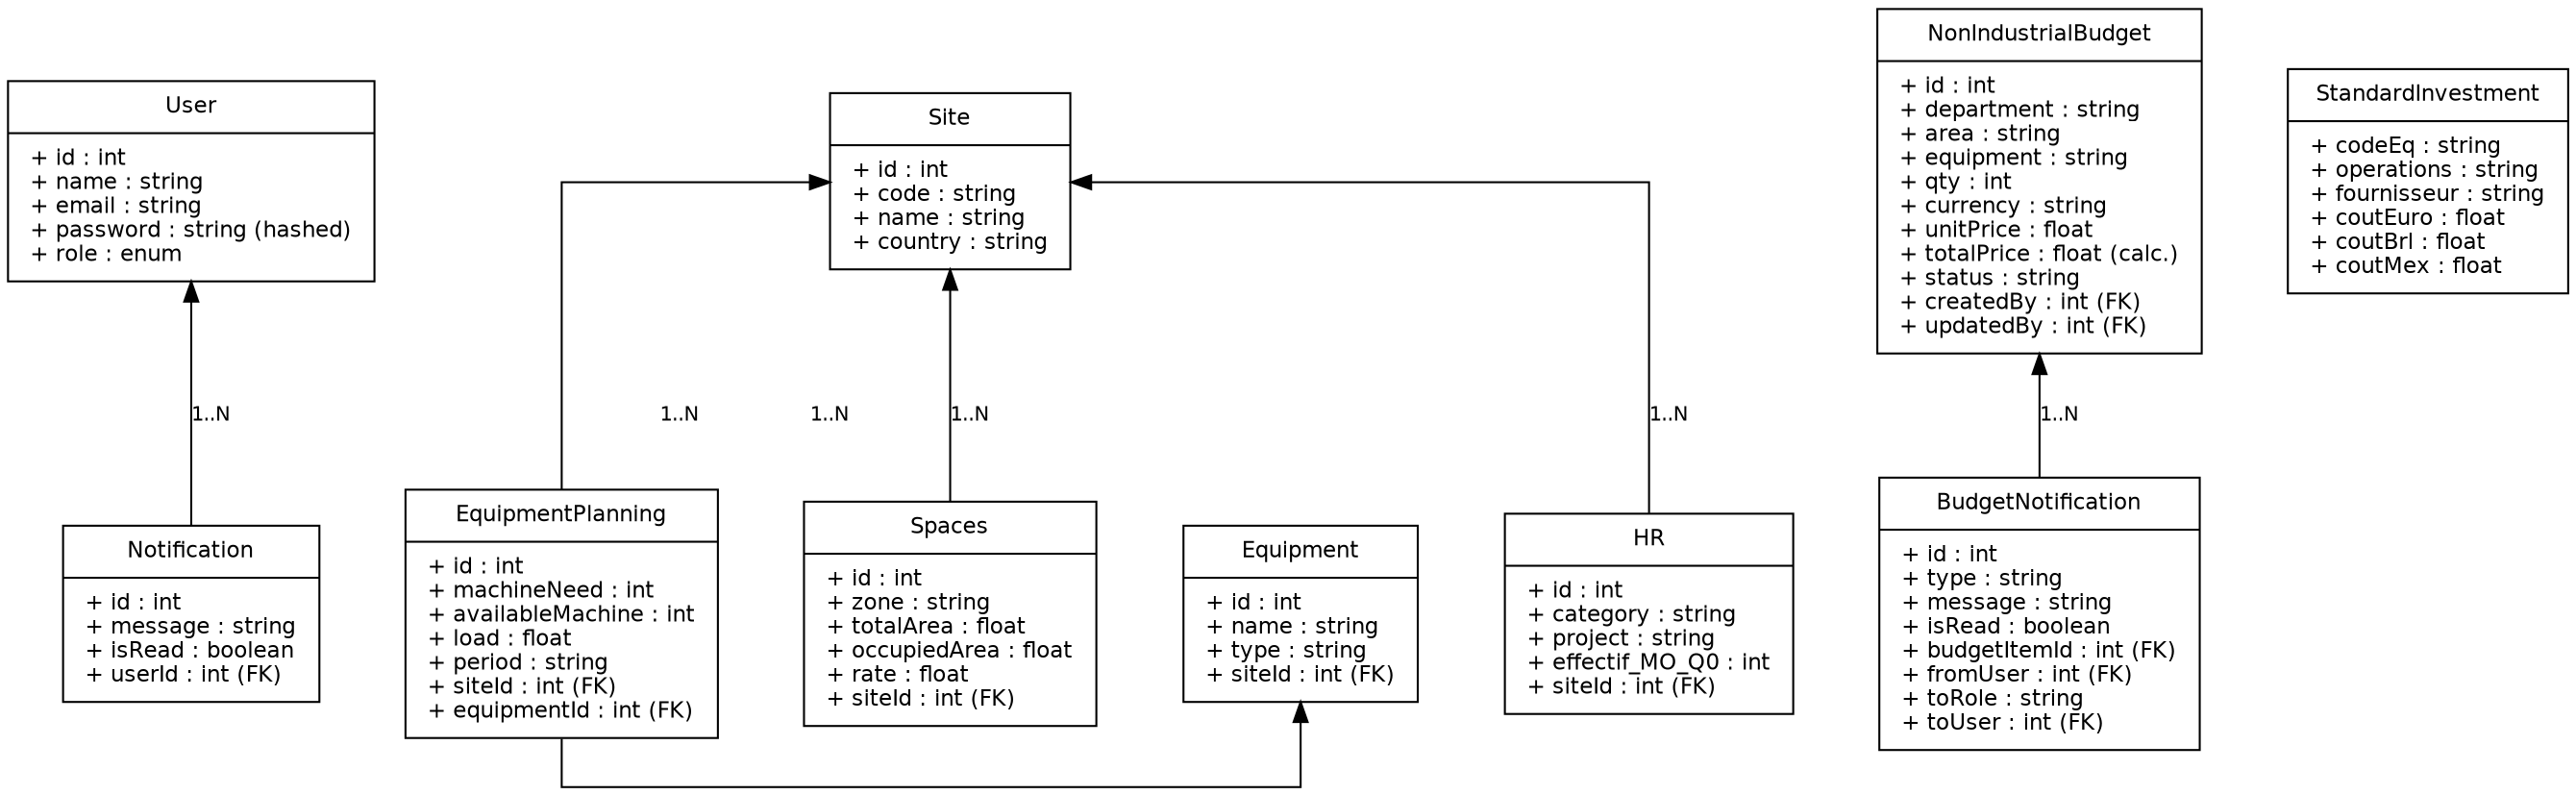
\includegraphics[width=\textwidth]{img/diagramme_classes_global.png} 
    \caption{Diagramme de classes global de l'application}
    \label{fig:class_diagram_global}
\end{figure}
\vspace{0.5cm}

\textbf{Analyse des relations (Cardinalités et Compositions) :}
Le diagramme illustre six relations structurelles majeures (implémentées en \textit{hasMany} et \textit{belongsTo} dans Sequelize). La classe \textbf{Site} est la clé de voûte de l'architecture multi-tenant :
\begin{itemize}
    \item \textbf{Site $\rightarrow$ EquipmentPlanning (1..N)} : Une usine effectue plusieurs centaines de prévisions sur une année. La suppression d'un site entraînerait logiquement la perte de ses prévisions (composition).
    \item \textbf{Site $\rightarrow$ Spaces (1..N)} et \textbf{Site $\rightarrow$ HR (1..N)} : Les espaces physiques et les effectifs sont strictement inféodés à leur site géographique (Mateur, Durango...).
    \item \textbf{Equipment $\rightarrow$ EquipmentPlanning (1..N)} : Chaque ligne de planning fait obligatoirement référence à une machine spécifique.
    \item \textbf{User $\rightarrow$ Notification (1..N)} : Un employé reçoit plusieurs alertes.
    \item \textbf{NonIndustrialBudget $\rightarrow$ BudgetNotification (1..N)} : L'historique des négociations tarifaires (Achat/Site Manager) est lié à l'article budgétaire concerné.
\end{itemize}

\textbf{Traçabilité des exigences :} chacun des besoins fonctionnels et non fonctionnels énumérés dans les sections précédentes a été systématiquement rattaché à une ou plusieurs User Stories du Backlog Général présenté ci-après, garantissant qu'aucune exigence exprimée lors des ateliers de spécification ne soit perdue lors du passage à la phase de développement. Cette traçabilité, bien que non matérialisée ici sous la forme d'une matrice formelle par souci de concision, a été maintenue tout au long du projet dans l'outil de suivi de tickets utilisé par l'équipe, chaque ticket de développement référençant explicitement l'identifiant de la User Story et, le cas échéant, le besoin non fonctionnel associé (par exemple, un ticket d'implémentation du middleware JWT référence à la fois l'US-01 et l'exigence de sécurité des accès).

\section{Le Backlog Général (Product Backlog)}
La transformation des spécifications UML en liste de tâches de développement s'est opérée lors des premières réunions avec le Product Owner. Nous avons adopté une priorisation basée sur la "valeur métier immédiate". Autrement dit, les modules permettant de débloquer le processus de planification locale ont reçu la priorité "Haute", la consolidation "Moyenne/Haute", tandis que le workflow budgétaire plus avancé a été planifié en priorité "Moyenne" pour la fin du projet. 

Concrètement, ce critère de priorisation découle d'une analyse simple mais structurante menée avec M. BOUCHOUICHA : une fonctionnalité est jugée prioritaire si son absence bloque totalement un usage métier existant (par exemple, sans authentification ni gestion des sites, aucun autre module ne peut fonctionner, d'où la priorité "Haute" des US-01 à US-03), tandis qu'une fonctionnalité vient enrichir un usage déjà partiellement possible autrement est jugée de priorité "Moyenne" ou "Basse" (le workflow budgétaire, bien qu'important, pouvait continuer à être géré de façon transitoire par courriel le temps que les modules de planification soient livrés en priorité). Cette logique de priorisation, proche dans l'esprit de la méthode MoSCoW (Must have, Should have, Could have, Won't have) sans en reprendre formellement le vocabulaire, a permis de garantir qu'à l'issue de chaque sprint, même interrompu prématurément, l'application livrée reste utilisable en l'état par au moins un profil d'utilisateur.

Le tableau \ref{tab:backlog} présente ce Backlog Général, constitué de 14 User Stories (US), qui ont guidé le travail de développement sur la période de mars à septembre 2026.

\begin{table}[h]
\centering
\begin{tabular}{|p{2cm}|p{8cm}|p{2cm}|p{2cm}|}
\hline
\textbf{ID US} & \textbf{Description (En tant que... je veux... afin de...)} & \textbf{Acteur} & \textbf{Priorité} \\ \hline
US-01 & En tant qu'utilisateur, je veux m'authentifier de manière sécurisée afin d'accéder au portail. & Tous & Haute \\ \hline
US-02 & En tant qu'admin, je veux gérer (CRUD) les utilisateurs et leurs rôles. & Admin & Haute \\ \hline
US-03 & En tant qu'admin, je veux paramétrer la liste des sites industriels. & Admin & Haute \\ \hline
US-04 & En tant que Site Manager, je veux importer un fichier Excel de mes équipements locaux. & Site Mgr & Haute \\ \hline
US-05 & En tant que Site Manager, je veux visualiser l'analyse de charge de mes machines (Load \%). & Site Mgr & Haute \\ \hline
US-06 & En tant que Site Manager, je veux importer et analyser mes besoins RH. & Site Mgr & Haute \\ \hline
US-07 & En tant que Site Manager, je veux importer et gérer mes espaces de production. & Site Mgr & Haute \\ \hline
US-08 & En tant qu'admin, je veux visualiser le dashboard consolidé mondial des Équipements. & Admin & Moyenne \\ \hline
US-09 & En tant qu'admin, je veux visualiser la consolidation des Espaces et des RH du groupe. & Admin & Moyenne \\ \hline
US-10 & En tant qu'acheteur, je veux consulter et mettre à jour les 2 colonnes de coûts du catalogue StandardInvestment. & Achat & Moyenne \\ \hline
US-11 & En tant que Site Manager, je veux créer et soumettre une demande de budget non-industriel. & Site Mgr & Moyenne \\ \hline
US-12 & En tant qu'acheteur, je veux modifier les 2 colonnes autorisées (prix unitaire et devise) d'une demande budgétaire soumise. & Achat & Moyenne \\ \hline
US-13 & En tant qu'utilisateur, je veux recevoir une notification temps réel lors d'une mise à jour sur mon budget. & Tous & Basse \\ \hline
US-14 & En tant qu'admin, je veux pouvoir exporter les données de budget en format Excel et PDF. & Admin & Basse \\ \hline
\end{tabular}
\caption{Backlog Général du projet}
\label{tab:backlog}
\end{table}

\textbf{Synthèse de planification :} Ce backlog de 14 User Stories a été réparti logiquement sur les 4 Sprints du projet. Le Sprint 1 a absorbé le socle (US-01 à 03). Le Sprint 2 s'est focalisé sur la planification locale (US-04 à 07). Le Sprint 3 a matérialisé la puissance d'agrégation mondiale et des standards (US-08 à 10). Enfin, le Sprint 4 a bouclé le périmètre avec le workflow de budgétisation collaborative (US-11 à 14).

\section{Règles de gestion et contraintes d'intégrité}
Au-delà des besoins fonctionnels et non fonctionnels formulés précédemment sous forme de phrases, plusieurs règles de gestion transversales, plus fines, ont émergé lors des ateliers de spécification et ont été appliquées de façon homogène sur l'ensemble des modules du système. Ces règles, bien que ne constituant pas des User Stories à part entière, conditionnent la validité de toute donnée entrant dans le système.

\begin{itemize}
    \item \textbf{Unicité du rattachement site-utilisateur :} un compte utilisateur de rôle Site Manager est obligatoirement rattaché à un unique site de production au moment de sa création par l'Admin. Ce rattachement conditionne l'ensemble du filtrage automatique appliqué aux requêtes de ce compte dans les modules de planification locale.
    \item \textbf{Non-négativité des grandeurs physiques et financières :} les champs \texttt{machineNeed}, \texttt{availableMachine}, \texttt{totalArea}, \texttt{occupiedArea}, \texttt{qty} et \texttt{unitPrice} ne peuvent jamais accepter de valeur négative, une contrainte vérifiée à la fois côté formulaire React (retour visuel immédiat) et côté modèle Sequelize (validation \texttt{min: 0}), afin d'empêcher toute incohérence de saisie même en cas de contournement de l'interface graphique.
    \item \textbf{Immuabilité du champ \texttt{totalPrice} :} ce champ n'est jamais directement saisissable par un utilisateur, quel que soit son rôle ; il est systématiquement recalculé par le serveur à partir de \texttt{qty} et \texttt{unitPrice}, garantissant qu'aucune incohérence entre le prix unitaire affiché et le total ne puisse survenir.
    \item \textbf{Traçabilité systématique des créateurs et modificateurs :} chaque enregistrement des tables \texttt{NonIndustrialBudget}, \texttt{EquipmentPlanning}, \texttt{Spaces} et \texttt{HR} conserve une référence vers l'utilisateur ayant créé la ligne (\texttt{createdBy}) et, le cas échéant, vers celui l'ayant modifiée en dernier (\texttt{updatedBy}), assurant l'imputabilité de toute donnée en cas de question ou de litige ultérieur sur son origine.
\end{itemize}

Ces règles de gestion, transversales à plusieurs modules, ont été centralisées dans des fonctions de validation réutilisables côté backend plutôt que dupliquées dans chaque contrôleur, réduisant le risque qu'une règle soit appliquée dans un module mais oubliée dans un autre lors d'une évolution future de l'application.

\section{Conclusion}
Ce deuxième chapitre nous a permis de structurer de manière rigoureuse les fondations du développement logiciel. En clarifiant le rôle exact de chaque acteur — notamment les limitations volontaires apportées au rôle Achat — et en listant exhaustivement les besoins fonctionnels (authentification JWT, import massif Excel, consolidation temps réel) et non fonctionnels (architecture 3-tiers, performances SQL, sécurité), nous avons sécurisé la trajectoire du projet. Les modélisations UML (cas d'utilisation et classes) ont prouvé que la conception de la base de données est parfaitement alignée avec les processus métier de COFAT. Le Backlog Général, fort de ses 14 User Stories, constitue désormais notre contrat de développement.

Les scénarios d'usage détaillés et les règles de gestion transversales présentés dans ce chapitre serviront également de référence constante lors de la description des interfaces réalisées dans les chapitres suivants : chaque écran présenté à partir du chapitre 3 pourra ainsi être directement rattaché à l'une des User Stories du backlog et à l'un des profils utilisateurs ici définis, garantissant une continuité de lecture entre la phase de spécification et la phase de réalisation technique du projet.

La prochaine étape, détaillée dans le chapitre suivant, plongera au cœur de la réalisation technique. Nous y argumenterons les choix des technologies et des frameworks, décrirons l'architecture logicielle retenue, avant de présenter les interfaces concrètes du Sprint 1, première brique fonctionnelle du portail web.
